\documentclass[a4paper]{article}
\usepackage{fullpage, titling, amsmath, footnote, listings, graphicx, subfig}
\makesavenoteenv{tabular}
\setlength{\droptitle}{-50pt}

\title{Machine Learning Assignment 2: Decision Trees}
\author{Group 31 \\ Chris Bates, Joe Slade, Andrew West, Thomas Wood}

\begin{document}
\maketitle
\section{Implementation Details}
Each test example is classified by all 6 decision trees. This process may
result in a single example being classed as multiple emotions. As every
example is required to be classed as a single emotion, a method of resolving
this was sought. 

Devising heuristics to solve this problem was difficult because complex
heuristics are likely to rely on the distribution of the underlying data
sets, rather than upon any application specific knowledge (ie, an
understanding of human emotions).

Instead, we chose a simpler, unbiased solution of picking a random emotion
from the set of possible classifications. When we tested using the given
data this was found to work reasonably well; in the rare case that a
conflict occurred, only two emotions were ever involved.

This solution is demonstrated in \emph{pick\_label} in
Figure~\ref{code:pick_label}.

Ambiguities may also occur when classifying examples if none of the six
trees recognise the example as their emotion.

We originally decided to return an unclassified result. However these 
reduced the overall efficacy of the system and it became apparent that it
was always worth guessing an emotion.

We next tried choosing a random emotion from among the six available and
although the system's precision was improved by this, analysis of the 
resulting confusion matrices suggested there was a better heuristic.

It was noted that the majority of these unclassified examples were in fact
examples of anger. Examination of Table 1 from the CBC Manual showed that
anger is also the most complex to classify under FACS. This combined with
the fact that comparatively few examples of anger were present in the
training data, meant that our system had greater difficulty in classifying
anger. Because of this, it was decided that in cases that no classification
could be found that it was most likely to actually be anger, so whenever our
system failed to classify an emotion the default of anger was returned.

\begin{figure}[h]
  \lstset{language=Matlab}
  \centering
  \begin{lstlisting}
  function [ label ] = pick_label( a,b,c,d,e,f )
  % Picks a random label from those that are set, or
  % guess 'anger' if no tree claims it
  label = 1;
  s = find([a b c d e f]);
  if size(s)
  pick = unidrnd(size(s,2));
  label = s(pick);
  end
  end
  \end{lstlisting}
  \caption{The code to resolve ambiguities}
  \label{code:pick_label}
\end{figure}

\section{Results}
Figure~\ref{table:confusion} shows the confusion matrix,
Figure~\ref{table:thing} shows the precision recall table, these show the
combined results after running for 10 folds.

It can be seen that emotions that have large numbers of examples in the sample
data are classified with great accuracy by the system, with happiness and
surprise almost always achieving perfect precision and recall. The lowest $F_1$
measures were recorded for fear and anger, which would be expected given that
these emotions have the fewest number of examples in the given data and are the
most complex emotions to classify according to FACS.

The $F_1$ measure for anger is significantly altered by our choice of a
heuristic for dealing with ambiguous cases, as explained above. Its precision
value is lowered by the larger number of false positives generated by
defaulting to anger in ambiguous cases, but increased by the even greater
proportion of true positive values which are now correctly classified, leading
to little overall change in precision. Its recall rate is however increased as
no extra false negatives are generated so the larger number of true positives
has a greater impact.

\begin{figure}
  \centering
  \begin{tabular}{c|cccccc}
    & Anger & Disgust & Fear & Happiness & Sadness & Surprise \\
    \hline
    Anger & 10 & 0 & 1 & 0 & 1 & 0 \\
  Disgust & 1 & 21 & 0 & 0 & 0 & 0 \\
     Fear & 2 & 0 & 5 & 0 & 0 & 0 \\
Happiness & 0 & 0 & 0 & 24 & 0 & 0 \\
  Sadness & 2 & 0 & 0 & 0 & 10 & 0 \\
 Surprise & 0 & 0 & 0 & 0 & 0 & 23 \\
  \end{tabular}
  \caption{Confusion Matrix}
  \label{table:confusion}
\end{figure}

\begin{figure}
  \centering
  \begin{tabular}{c|cccc|ccc}
    Emotion & TP & TN & FP & FN & Recall & Precision & $F_1$ \\
    \hline
    Anger & 10 & 83 & 5 & 2 & 0.833 & 0.667 & 0.741 \\
  Disgust & 21 & 78 & 0 & 1 & 0.955 & 1.000 & 0.977 \\
     Fear & 5 & 92 & 1 & 2 & 0.714 & 0.833 & 0.769 \\
Happiness & 24 & 76 & 0 & 0 & 1.000 & 1.000 & 1.000 \\
  Sadness & 10 & 87 & 1 & 2 & 0.833 & 0.909 & 0.870 \\
 Surprise & 23 & 77 & 0 & 0 & 1.000 & 1.000 & 1.000 \\
  \end{tabular}
  \caption{Average recall, precision rates and $F_1$ value per class}
  \label{table:thing}
\end{figure}

\section{Pruning}
The prune\_example function takes a set of AUs and the labels for that data,
and builds a decision tree using MATLAB's built in function \emph{treefit}.

Error rates are calculated for trees of increasing depth according to two
metrics, resubstitution and 10-fold cross-validation, and the results
plotted on two graphs.

Up until a tree size of 6, both cross-validation and resubstition have the
same error rates at each depth. Beyond this point, resubstitution shows
continued falling error rates with deeper trees, whilst cross-validation
shows an increased error rate.

The resubstitution method consistently underestimates the error because it
tests using the same data that the tree learned with, this is essentially
using a perfect training set - it is identical to the population. We
therefore expect there to be no error at the maximum depth, unless the
population contains inconsistent data.

The cross-validation method reserves a section of the input for use as a
testing dataset and the tree is trained using the remainder of the input.
This allows us to detect over-fitting of the tree to the training data as it
is tested against an unseen data set.

Over-fitting occurs when a tree is trained for too long or trained upon an
unrepresentative set of data as it has become too specialised and therefore
misses more general examples.

The point at which over-fitting starts to occur can be seen on the
cross-validation graph at the minimum, and that is the depth to which the
tree should be pruned to preserve accuracy.

It is not possible to detect over-fitting on the resubstitution graph as it
presents an overly-optimistic view of the error rate as the tree depth
increases.

\begin{figure}[p]
  \centering
  \subfloat[Anger]{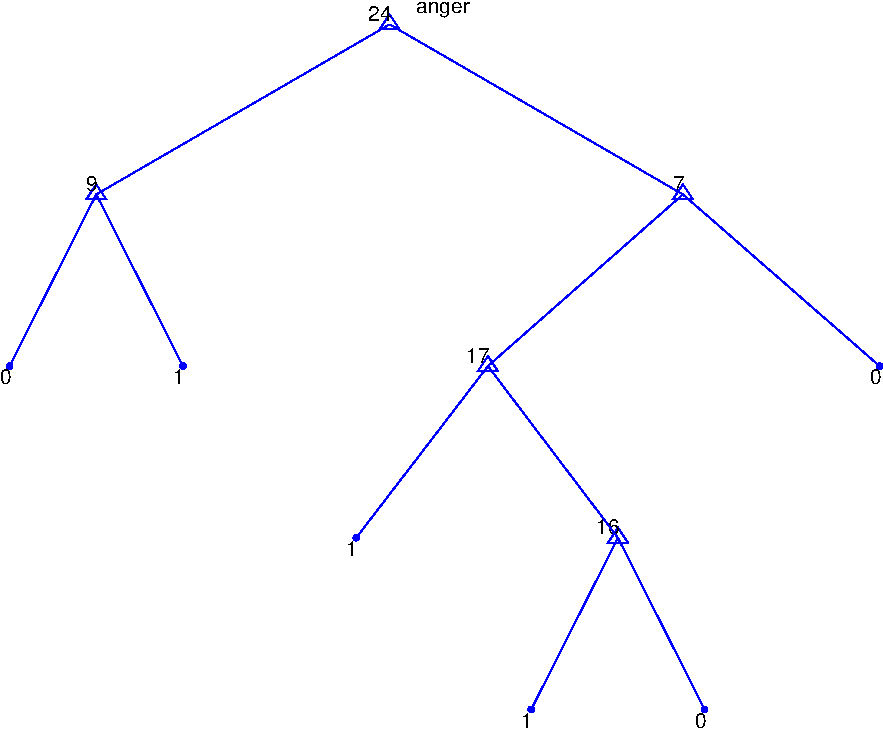
\includegraphics[width=0.3\textwidth]{graph-anger}}
  \subfloat[Disgust]{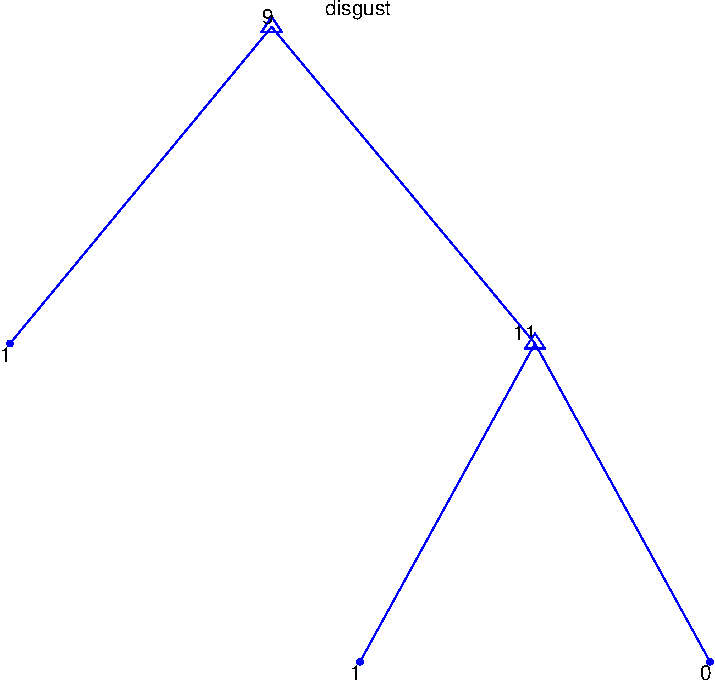
\includegraphics[width=0.3\textwidth]{graph-disgust}}
  \subfloat[Fear]{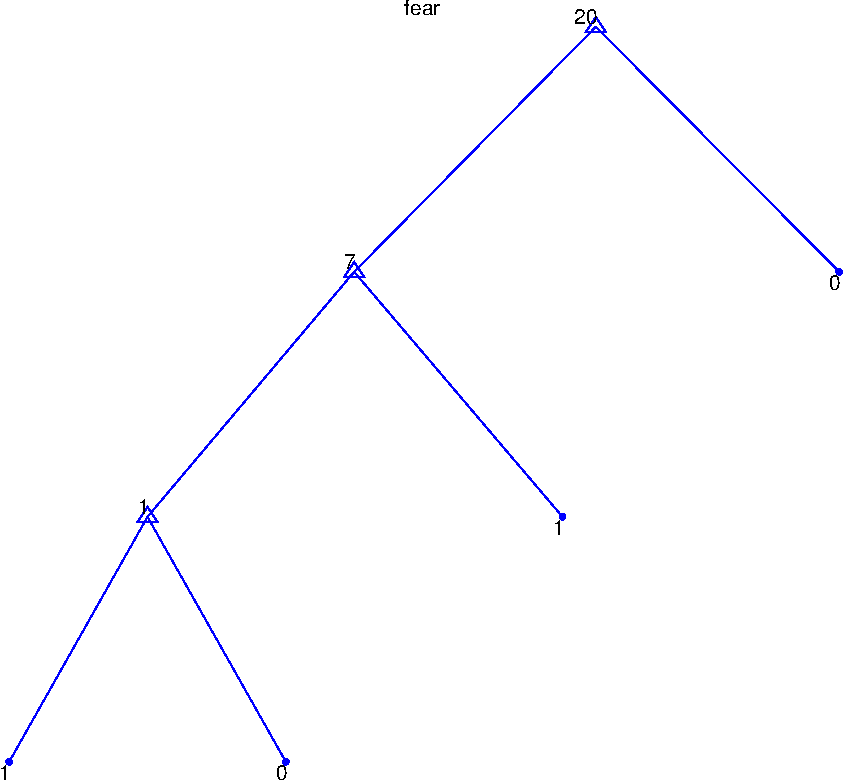
\includegraphics[width=0.3\textwidth]{graph-fear}}
  \\
  \subfloat[Happiness]{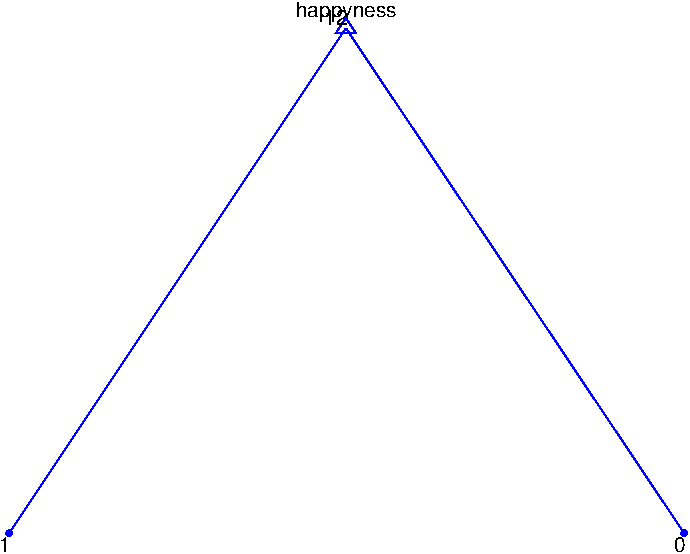
\includegraphics[width=0.3\textwidth]{graph-happyness}}
  \subfloat[Sadness]{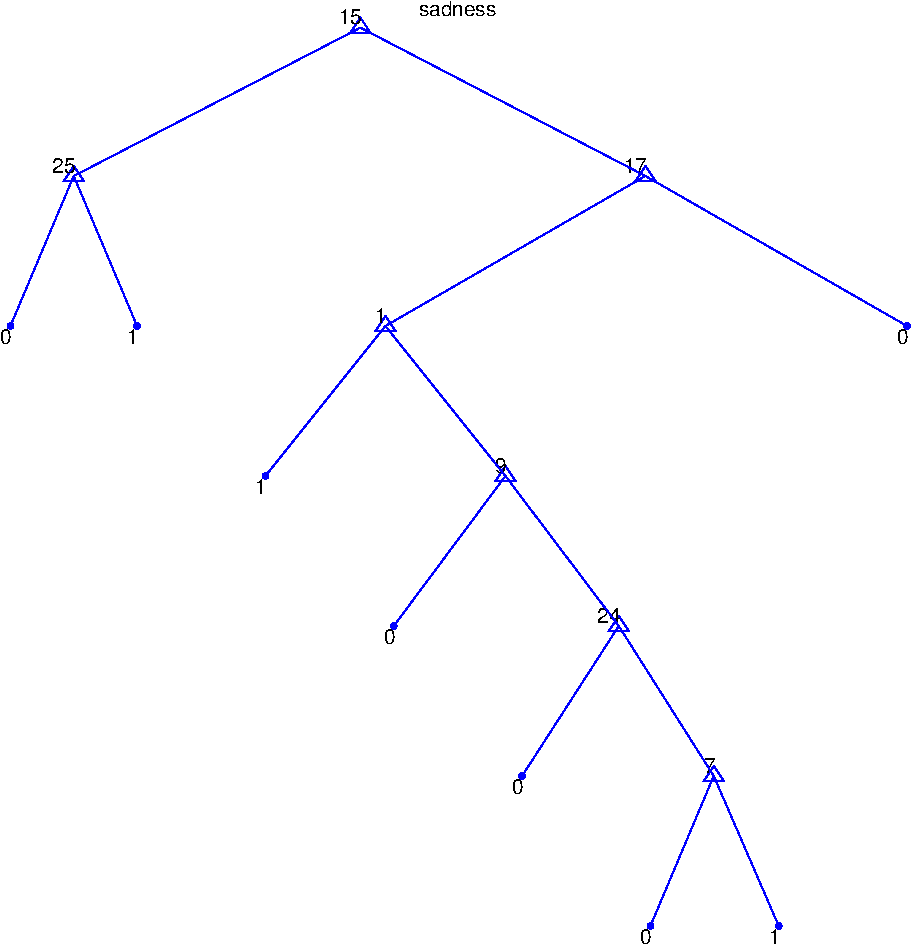
\includegraphics[width=0.3\textwidth]{graph-sadness}}
  \subfloat[Surprise]{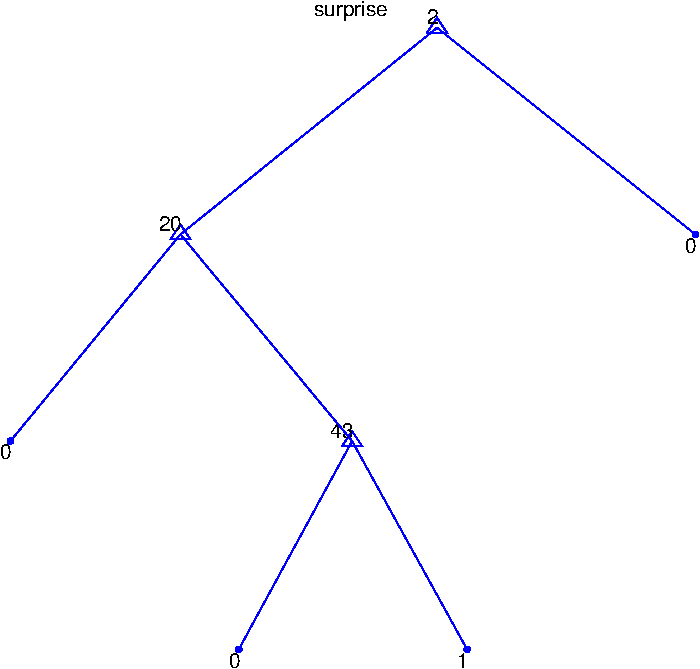
\includegraphics[width=0.3\textwidth]{graph-surprise}}
  \caption{Generated decision trees for the full dataset}
\end{figure}

\begin{figure}[p]
  \centering
  \subfloat[Cross-validation]{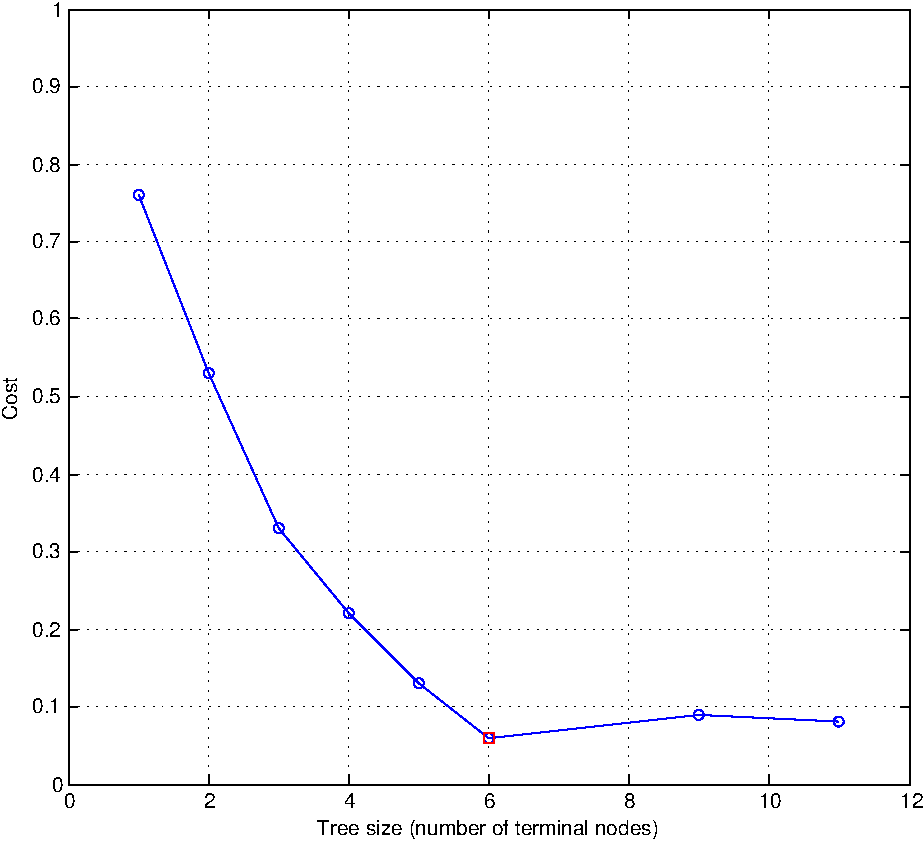
\includegraphics[width=0.45\textwidth]{graph-overfitting-1}}
  \subfloat[Resubstitution]{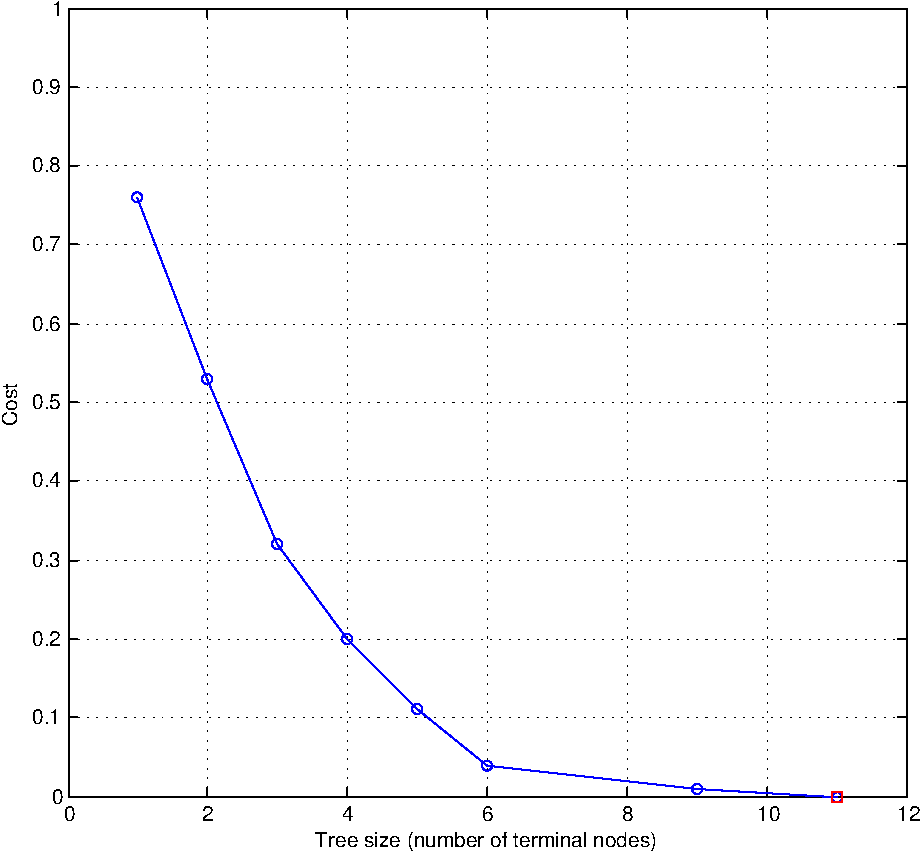
\includegraphics[width=0.45\textwidth]{graph-overfitting-2}}
  \caption{Tree-depth/Error-rate graphs}
\end{figure}

\end{document}

